\newthought{\textbf{Nadzura Kumaira - 2020903430030 - TRKJ 3B}}

\newday{\textbf{1 Desember 2022}- Instalasi Apache Hadoop}
\begin{enumerate}
\item Kendala dan Solusi
\newline berada di perintah hadoop version dimana ketika dilakukan perintah itu tidak keluar,tapi saya membuat ulang dan akhirnya bisa

\item Kesimpulan
\newline jangan ada perintah yang ketinggalan karena itu membuat error.

\begin{figure}[!ht]
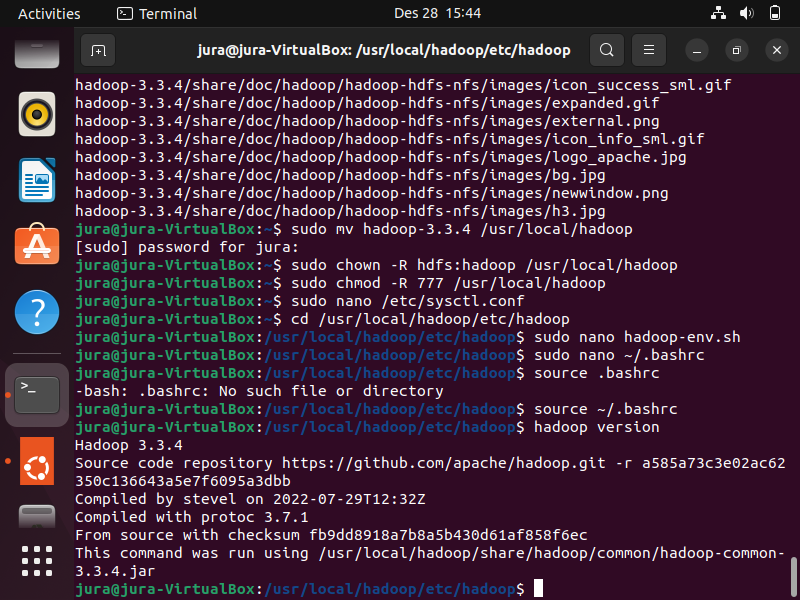
\includegraphics[width=\textwidth]
{NadzuraKumaira/hadoop version}
\caption{hasil dari hadoop version}
\label{gam:perkuliahan-25-11}
\end{figure}
\end{enumerate}

\newday{\textbf{2 desember 2022}}
\begin{enumerate}
\item Kendala dan Solusi
\item Kesimpulan
\end{enumerate}

\newday{\textbf{8 desember 2022}}
\begin{enumerate}
\item Kendala dan Solusi
\item Kesimpulan
\end{enumerate}

\newday{\textbf{9 desember 2022}}
\begin{enumerate}
\item Kendala dan Solusi
\item Kesimpulan
\end{enumerate}

\newday{\textbf{15 desember 2022}}
\begin{enumerate}
\item Kendala dan Solusi
\item Kesimpulan
\end{enumerate}

\newday{\textbf{16 desember 2022}}
\begin{enumerate}
\item Kendala dan Solusi
\item Kesimpulan
\end{enumerate}

\newday{\textbf{22 desember 2022}}
\begin{enumerate}
\item Kendala dan Solusi
\item Kesimpulan
\end{enumerate}

\newday{\textbf{23 desember 2022}}
\begin{enumerate}
\item Kendala dan Solusi
\item Kesimpulan
\end{enumerate}